\documentclass[12pt,a4paper,olive]{bbe}
\usepackage{blindtext}
\usepackage{fancyvrb}
\begin{document}
			
	\chapter{Algorithmic Analysis}
	\section{Correctness}
	A problem X is defined as an ordered (q,a) set where 'q' is a question and 'a' is an answer, written mathematically as: 
 
	
	$$X={((q(x),a(x)) | x \exists D)}$$
	With a 'D' arbitrary set of data.
	
	Q(x) is the set of questions:
	$$ Qx = {q | (q, a) \exists X} $$

	and a set of questions is solved by an algorithm 'A' if
	$$ (\forall q \exists Px | A[q] = a :(q, a) \exists X) $$

	Besides all of this, the size of a question is written as 
	\it|q|=i\it, the difficulty of
	a question is usually proportional to its size.

	An algorithm is considered correct if it solves a problem given A input, resulting in a desired B output in all possible cases.
	
	\section{Complexity}
	Algorithmic complexity is the approximated cost of an algorithm when running on a machine capable of computing. This kind of analysis can be quantified in time, memory, and even operational costs.

	\begin{remark}
	The method to define and value algorithms must be independent of programming language, architecture, and even more broadly, of the specific machine the algorithm runs on. This implies we don't take into account computational problems, such as compilation or, in interpreted languages, the interpretation into bytecode of the algorithm, for this doesn't concern the algorithm, but rather factors external to it.   
	\end{remark}

	\subsection{R-Complexity}
	R is the class of decision problems solvable by a Turing machine. The main idea of it is defining a sum of the costs inside of the machine according to the operations realized by the algorithm. Resulting mathematically in the total cost of the algorithm's execution. However, R-Complexity is generally hard to compare between programming languages and individual machines because of the dependance of the result in constants.

	given this definition, take as an example: 
	\bigskip
	\bigskip

	\begin{verbatim}
	#Python pseudocode, take a list and copy it into another.
	def Solution(list nums): 
	    answer = [] # <-- R = C1 + C2
	    for i in list: # <-- R = nC9
	        answer.append(i) # <-- <-- R = nC8 
	    return answer
	\end{verbatim}

	And therefore, the R-Complexity of this equation is $$R_n=C1+C2*n(C9+C8)$$ 

	However, even though this algorithm might have such R-Complexity, different implementations of this 
	same Algorithm, where the solution is expressed even slightly different, could have completely different
	R-Complexity equations.

	Take as an example:
	\begin{verbatim}
		#Python pseudocode, take a list and copy it into another.
		def solution(List): 
		answer = [] 				 # <-- R = C1 + C2
		for i in range(0,len(List)): # <-- R = C1 + (n + 1)C3 + (n+1)C4 + nC5
		    current = List[i]		 # <-- R = nC1 + nC6
		    answer.append(current)   # <-- R = nC7 + nC8
		return answer
	\end{verbatim}

	this implementation is a different algorithm that solves the exact same problem, and which R-Complexity can be
	defined as:
	$$ R_n = 2C_1 + C_2 + C_3 + C_4 + n(C_1 + C_3 + C_4 + C_5 + C_6+ C_7+ C_8) $$
	This is a fairly different, much longer equation, which includes a lot more constants and a bit more complex to compute
	Given this, sometimes R-Complexity might end up being fairly dependant on implementation when different solutions are presented.
	\subsection{Complexity Order}
	be it 'f' and 'q' functions such as: $f,g : \mathbb{N} \rightarrow \mathbb{R}$

	we can affirm that f is of equal or lesser order to g if:
	$$ ( \exists c, k \exists \mathbb{N} |: (\forall m \exists \mathbb{N} | k \le m : f(m) \le cg(m) ) ))$$

	and we can write it as: 
	$$f = \mathbb{O}(g) \land f(n) = O(g(n))$$
	
	'O' induces a partial order on functions such as $$\mathbb{N} \rightarrow \mathbb{R}$$ and 
	is an equivalence relation over that same group of functions. 

	\subsubsection{Order Theorems}
	\begin{itemize}
		\item Constant rule: $$(\forall c  \exists  N | : cf = O(f))$$
		\item {
			Sum rule: $$ f + g = O(max(f,g)) $$
			\subparagraph*{proven as:}
			
			}
		\item {
			Product rule: $$ f = O(r) \land g = O(s) \longrightarrow fg = O(rs) $$
			\subparagraph*{proven as:}
			
			}
	\end{itemize}

	\subsubsection{Order classification examples}
	\begin{enumerate}
		\item $$2n^5 = O(n^5)$$
		\item $$2n^5 + 4n = O(n^5) $$
		\item $$ (2n^5 + 4n)^2 = O(n^{10})$$
		\item $$(n+1)^2 = O(n^2)$$
	\end{enumerate}

	\subsection{Complexity orders}
	Complexity orders are classified as follows, according to big O notation.
	\begin{itemize}
		\item {
			\subparagraph*{$$O(1)$$} 
		Constant: Execution time doesn't depend on the size of the input
		} 
		\item {
			\subparagraph{$$O(log(n))$$}
		Logarithmic: Execution time grows slower than the input size, Ex: binary search
		}
		\item {
			\subparagraph{$$O(n)$$}
		Linear: Execution time grows at the same rate as the input size, Ex. Unordered array search 
		}
		\item {
			\subparagraph{$$O(n log(n))$$}
		Log-Linear: Execution time grows at the same rate as the input size but does O(log(n)) operations per item
		}
		\item {
			\subparagraph{$$O(n^2)$$}
		Quadratic: Execution time grows at a linear rate related to the input size, but requires a linear operation per item in the input.
		}
		\item {
			\subparagraph{$$O(2^n)$$}
		Exponential: Execution time grows exponentially compared to the input
		}
	\end{itemize}


	\chapter{Recursion}
	Recursion in this context is defined as a finite expression that implies
	succesion.
	\section{Recursive Equation}
	A recursive equation describes the value of the element of a succesion 
	parting from previous elements of that specific succesion. These can be defined
	in either a linear or non-linear way, depending on the problem to be solved by
	this recursive algorithm.
	\section{Linear Equations}
	\subsection{Homogeneous Linear Recursive Relation}
	A Homogeneous linear recursive relation is a relation that can be defined
	in mathematical terms as a relation that could be expressed by the formula:

	$$ \sum_{i = 0}^{k} a_i f(n-1) = 0 $$

	and that includes a characteristic polinomial that can be expressed as:
	$$\sum_{i = 0}^{k} a_i \lambda^(n-1)$$

	\subsection{Non-linear Recursive Relation}
	A non linear recursive relation is a relation we can explain as defined by the formula
	$$ \sum_{i = 0}^{k} a_i f(n-1) = \mathbb{R} $$

	where the solution is different from zero.


	\subsection{Examples}

	We suppouse a $T(n)$ of the form:
	$$ T(n) = \sum_{i=0}^{k} aT(n-i)=g(n) $$
	we would have the solution:
	$$T(n) = h(n)+P(n)$$
	Where:

	\begin{itemize}
		\item $g(n)=c \rightarrow P(n)=C_0$
		\item $ g(n) = Cn + c' \rightarrow P(n) = C_0n+C_1 $
	\end{itemize}

	\subsubsection{Example 1}
	For the case in which T(n) is
	$$ T(n) = \begin{cases} 
	2\\
	3n+3T(n-1)
	\end{cases}  $$
	find:
	\begin{itemize}
		\item h(n)
		\item p(n)
	\end{itemize}
	\paragraph*{Solution}
	to find h(n), first we define the first characteristic polynomial as:
	$$
	\lambda -3=0
	$$
	$$
	\lambda = 3
	$$

	And the second as:
	$$ 2 =  C_0^1 3^1$$
	$$ \frac{2}{3} = C_0^1 $$


	And therefore, we conclude
	h(n) = $C_0^1 3^n$ and h(n) = $2 * 3^{n-1}$
	
	\section{Non-Linear Equations}

	\subsection{Recurrent non-linear equations.}
	A recurrent non-linear equation is,

	\subsubsection{Recursion Tree}
	this is a graphical method for solving non-linear equations. The 
	solution of this method is defined by the recurrent decomposition of
	a specific mathematical expression. Arriving to 
	
	\subsubsection{Substitution Method.}

	\subsubsection{Master Method.}

	\chapter{Divide and Conquer}
	Divide and Conquer is a programming technique based on the
	division of a larger problem into smaller, more manageable
	problems.
 
	\chapter{Graphs}
	A graph is a data structure defined by non-linearity. and even though
	generally considered more abstract than other options for data representations,
	it allows us to work with problems that would be otherwise a lot harder, 
	\section{Ordered Graphs}
	\section{Unordered Graphs}
	
	\section{Graph problems}
	
	\subsection{BFS}

	\subsubsection{pseudocode}
	\begin{verbatim}
		#Python pseudocode for BFS
		def bfs(adj, s):
		    visited = [False for v in adj]
		    queue = [s]
		    while 0 < len(queue)
		        current_node = queue.pop(0)
		        if not visited[current_nod]:
		            visited[current_nod] = True
		            for n in adj[current_nod]:
		                queue.append(n)
		            
	\end{verbatim}
	\subsection{Cycle Detection}
	\subsection{Connected components}
	\subsection{Topologic orders}

	\chapter{Greedy Algorithms}
	A greedy algorithm is an algorithm that selects the locally best option
	every time that it has to take a decision. Usually when talking about greedy
	algorithms we have to think about two main components:

	- Optimal substructures: greedily solving the problem requires
	being able to greedily solve it, the structure of the problem must
	allow it.

	- Greedy selection: As said beforehang, we must be able to solve this
	problem by selecting the best option every single time, without nescessairly
	caring about it's implications.

	\section{Minimum Spanning Trees}
	A minimum spanning tree is a tree derived from another graph. (Let's remember the
	definition of a tree from chapter 4, in case you're a bit confused by what that
	means.) this is an algorithm that has to work on a weighed graph to work. Any tree that
	derives from the graph can be considered a 'spanning tree', however, the one with the
	minimum sum of weighs is considered the 'minimum spanning tree'.

	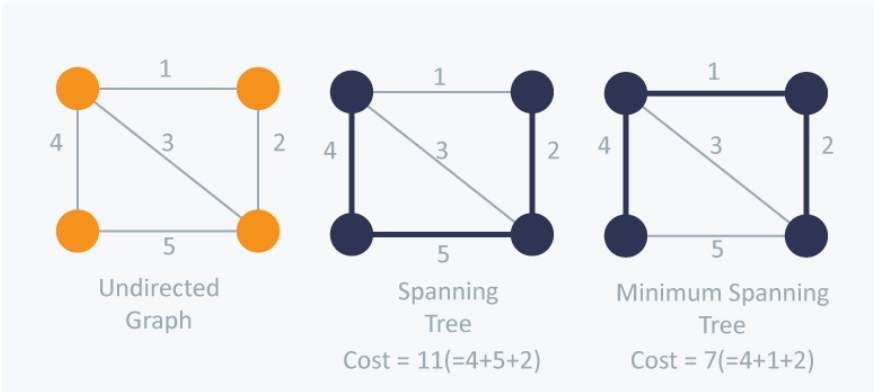
\includegraphics[scale=0.55]{pics/mst.png}

	It is possible that we might find ourselves on a 
	
	\subsection{Prim Algorithm}

	\subsection{Kruskal Algorithm}
	Kruskal's algorithm tries to solve the minimum spanning tree problem
	via...

	An example of Kruskal pseudocode would be:
	
	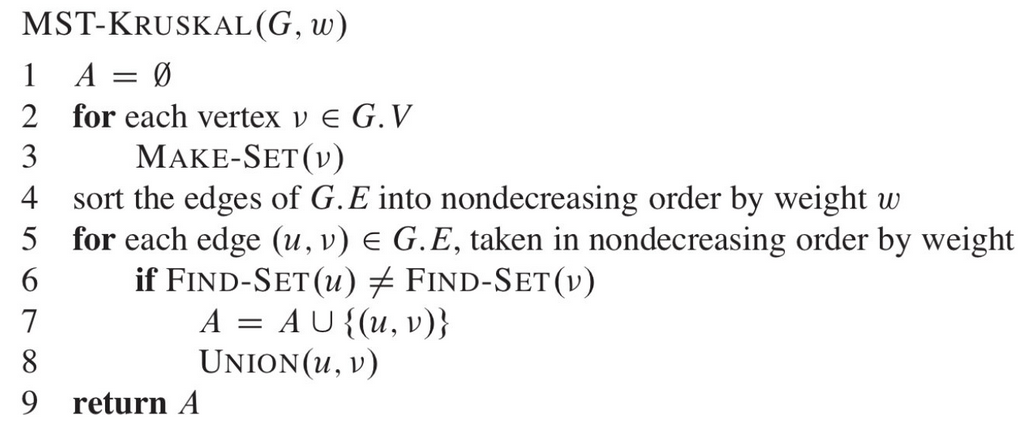
\includegraphics[scale=0.4]{pics/kruskal.png}
\end{document}